\documentclass{beamer}
\usetheme{AnnArbor}
\usepackage{graphicx}
\graphicspath{{pics/}}
\usepackage{amsmath}
\usepackage{amssymb}
\usepackage{framed}
\usepackage{tikz}
\usepackage[]{xcolor}
\usepackage[most]{tcolorbox}
\usepackage{pgfplots}
\pgfplotsset{compat=1.18}
\usepackage{blkarray}
\setbeamercolor{mycolorbox}{%
  bg=yellow!20,   % background color (20% yellow)
  fg=black      % foreground (text) color
}
\usefonttheme[onlymath]{serif}

\newtcolorbox{solutionblock}{
  colback=yellow!5,        % Background color: light yellow
  colframe=orange!80!black, % Frame color: dark orange
  title=Solution,
  fonttitle=\bfseries
}

\title{Introduction to Functions}
\author{Nithin}
\institute{}
\date{\today}
\begin{document}
\begin{frame}
  \titlepage
\end{frame}
\begin{frame}
  \tableofcontents
\end{frame}
\section{Slopes and Average Rate of Change}

% Slide: Motivation and Overview
\begin{frame}{Motivation: Why Study Change?}
  \begin{itemize}
    \item Calculus explores how quantities change and provides tools for modeling these changes.
    \item Functions link inputs ($x$) to outputs ($y=f(x)$); we investigate how $y$ varies as $x$ moves over an interval.
    \item Real-world example: Predicting economic indicators, modeling speeds, and more.
  \end{itemize}
\end{frame}

% Slide: What is a Secant Line?
\begin{frame}{What is a Secant Line?}
  \begin{block}{Definition}
    A \emph{secant line} is a straight line that passes through two points on a curve.
  \end{block}
  \begin{itemize}
    \item Given two points $(a,f(a))$ and $(b,f(b))$ on the curve $y=f(x)$
    \item The secant line connects these two points
    \item Its slope represents the average rate of change over the interval $[a,b]$
    \item Unlike the curve itself, the secant line has constant slope
  \end{itemize}
  \vspace{1ex}
  \begin{center}
    \textbf{Secant line slope} = $\dfrac{\text{rise}}{\text{run}} = \dfrac{f(b)-f(a)}{b-a}$
  \end{center}
\end{frame}

% Slide: Why is Secant Line Slope Called "Average Rate of Change"?
\begin{frame}{Why ``Average Rate of Change''?}
  \begin{itemize}
    \item The function $f(x)$ may have varying rates of change at different points
    \item Between points $a$ and $b$, the function might:
    \begin{itemize}
      \item Increase rapidly at some points
      \item Increase slowly at others
      \item Even decrease temporarily
    \end{itemize}
    \item The secant line slope $\dfrac{f(b)-f(a)}{b-a}$ captures the \textbf{net change} over the entire interval
    \item It ``averages out'' all the local variations to give one representative rate
  \end{itemize}
  \vspace{1ex}
  \begin{center}
    \textbf{Think of it as:} ``If the function changed at a constant rate from $a$ to $b$, what would that rate be?''
  \end{center}
\end{frame}

% Slide: Defining Average Rate of Change
\begin{frame}{Average Rate of Change}
  \begin{block}{Definition}
    For a function $f(x)$ on interval $[a,b]$, the \emph{average rate of change} is
    \[ 
      \frac{f(b)-f(a)}{b-a},
    \]
    which geometrically represents the slope of the secant line between $(a,f(a))$ and $(b,f(b))$.
  \end{block}
  \begin{itemize}
    \item Rise: $f(b)-f(a)$
    \item Run: $b-a$
    \item Secant line smooths out fluctuations; reports overall trend.
  \end{itemize}
\end{frame}

% Slide: Graphical Illustration
\begin{frame}{Graphical Illustration}
  \begin{columns}
    \column{0.6\textwidth}
      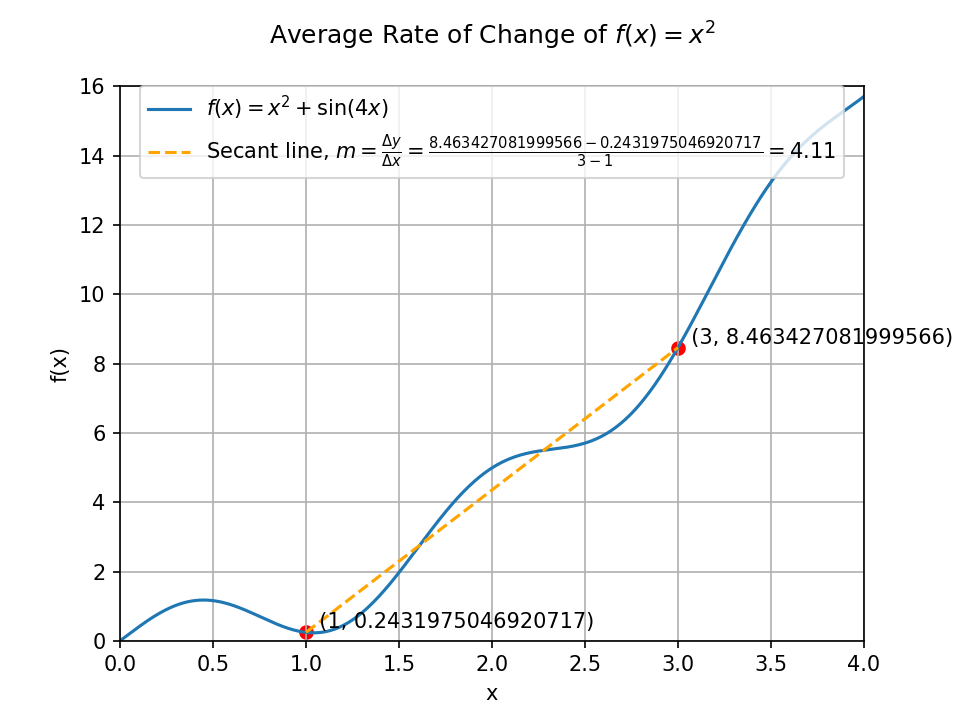
\includegraphics[width=\textwidth]{figures/avg_rate_of_change.png}
    \column{0.4\textwidth}
      \begin{itemize}
        \item Focus on interval $[1,3]$ on the curve $y=f(x)$.
        \item Secant line (in orange) joins $(1,f(1))$ and $(3,f(3))$.
        \item Its slope measures the average change in $y$ per unit change in $x$.
      \end{itemize}
  \end{columns}
\end{frame}

% Slide: Problem – Trivandrum to Chennai Average Speed
\begin{frame}{Example: Trivandrum to Chennai Journey}
  \begin{columns}
    \column{0.5\textwidth}
      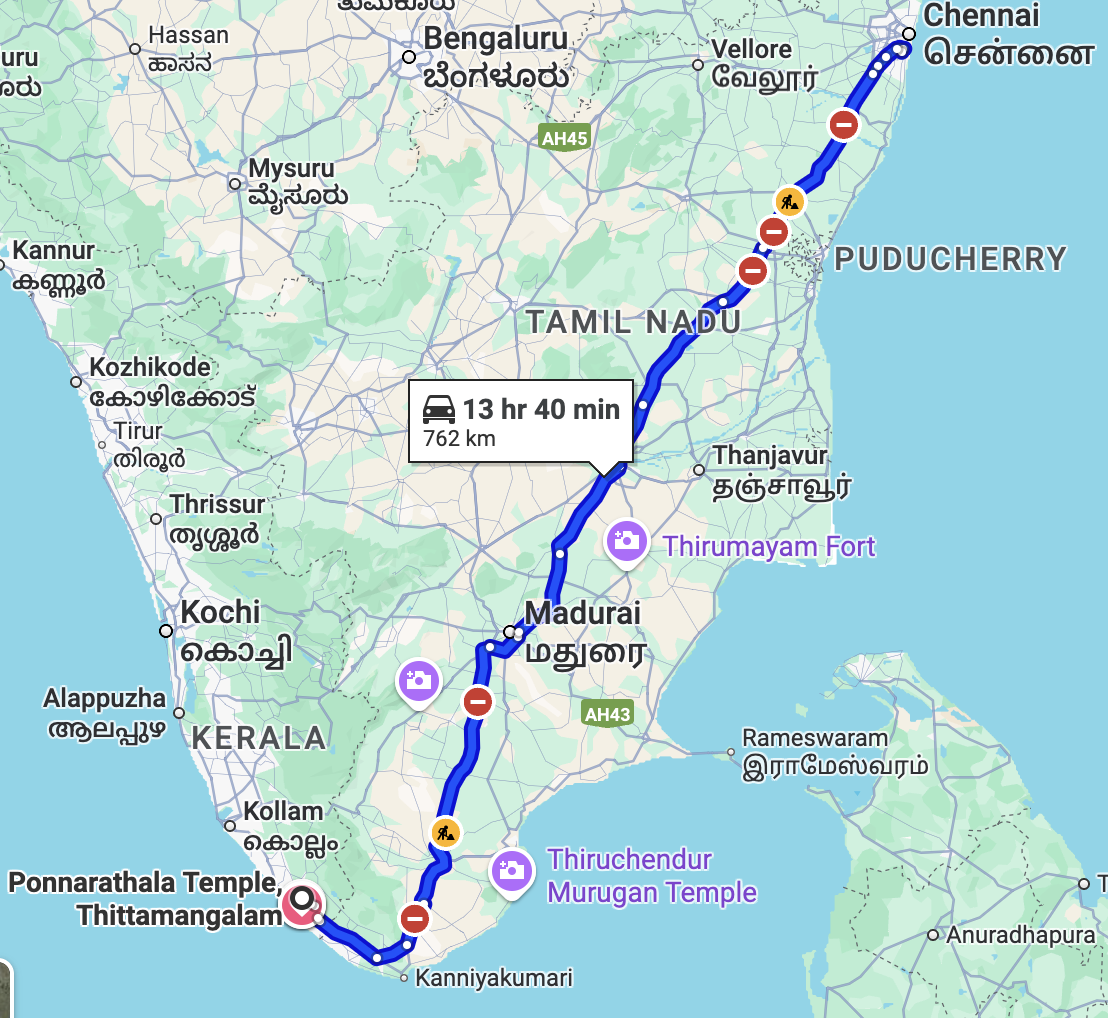
\includegraphics[width=\textwidth]{figures/trivandrum_chennai_map.png}
    \column{0.5\textwidth}
      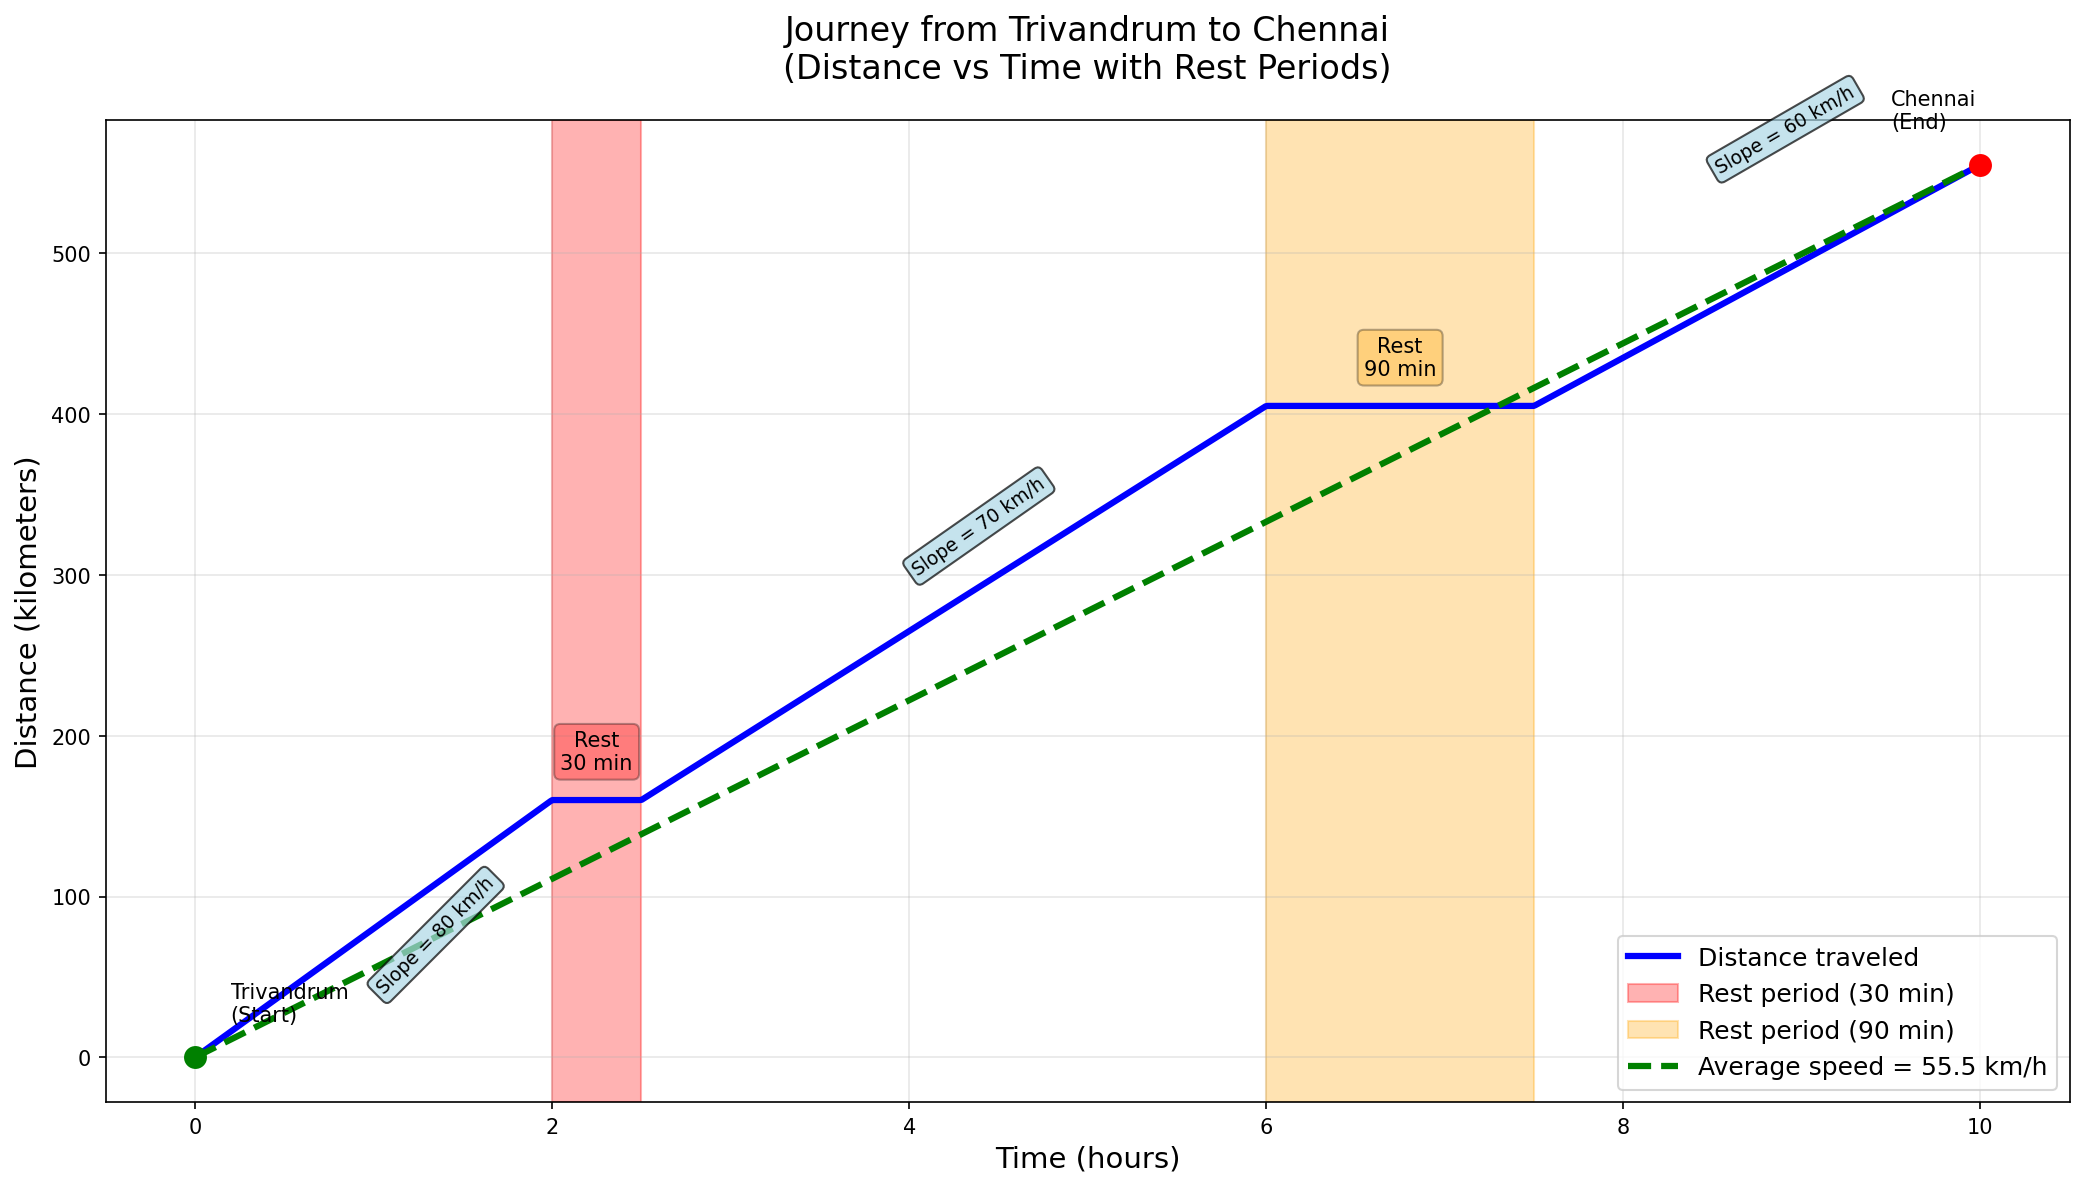
\includegraphics[width=\textwidth]{figures/trivandrum_chennai_journey.png}
  \end{columns}
  \vspace{1ex}
  \begin{itemize}
    \item Total distance: 762 km
    \item Total time (including stops): 15 hours
    \item Average speed: $\dfrac{762}{15}\approx50.8$ km/h
  \end{itemize}
\end{frame}
\begin{frame}
  \begin{solutionblock}
    Average speed $=\dfrac{\text{distance}}{\text{time}}=\dfrac{762}{15}\approx50.8\text{ km/h}$.  
  This illustrates how the secant slope over an interval gives overall performance even with rest periods.
  \end{solutionblock}
\end{frame}

% Slide: Sensitivity to Rounding
\begin{frame}{Rounding and Accuracy}
  \begin{columns}
    \column{0.58\textwidth}
      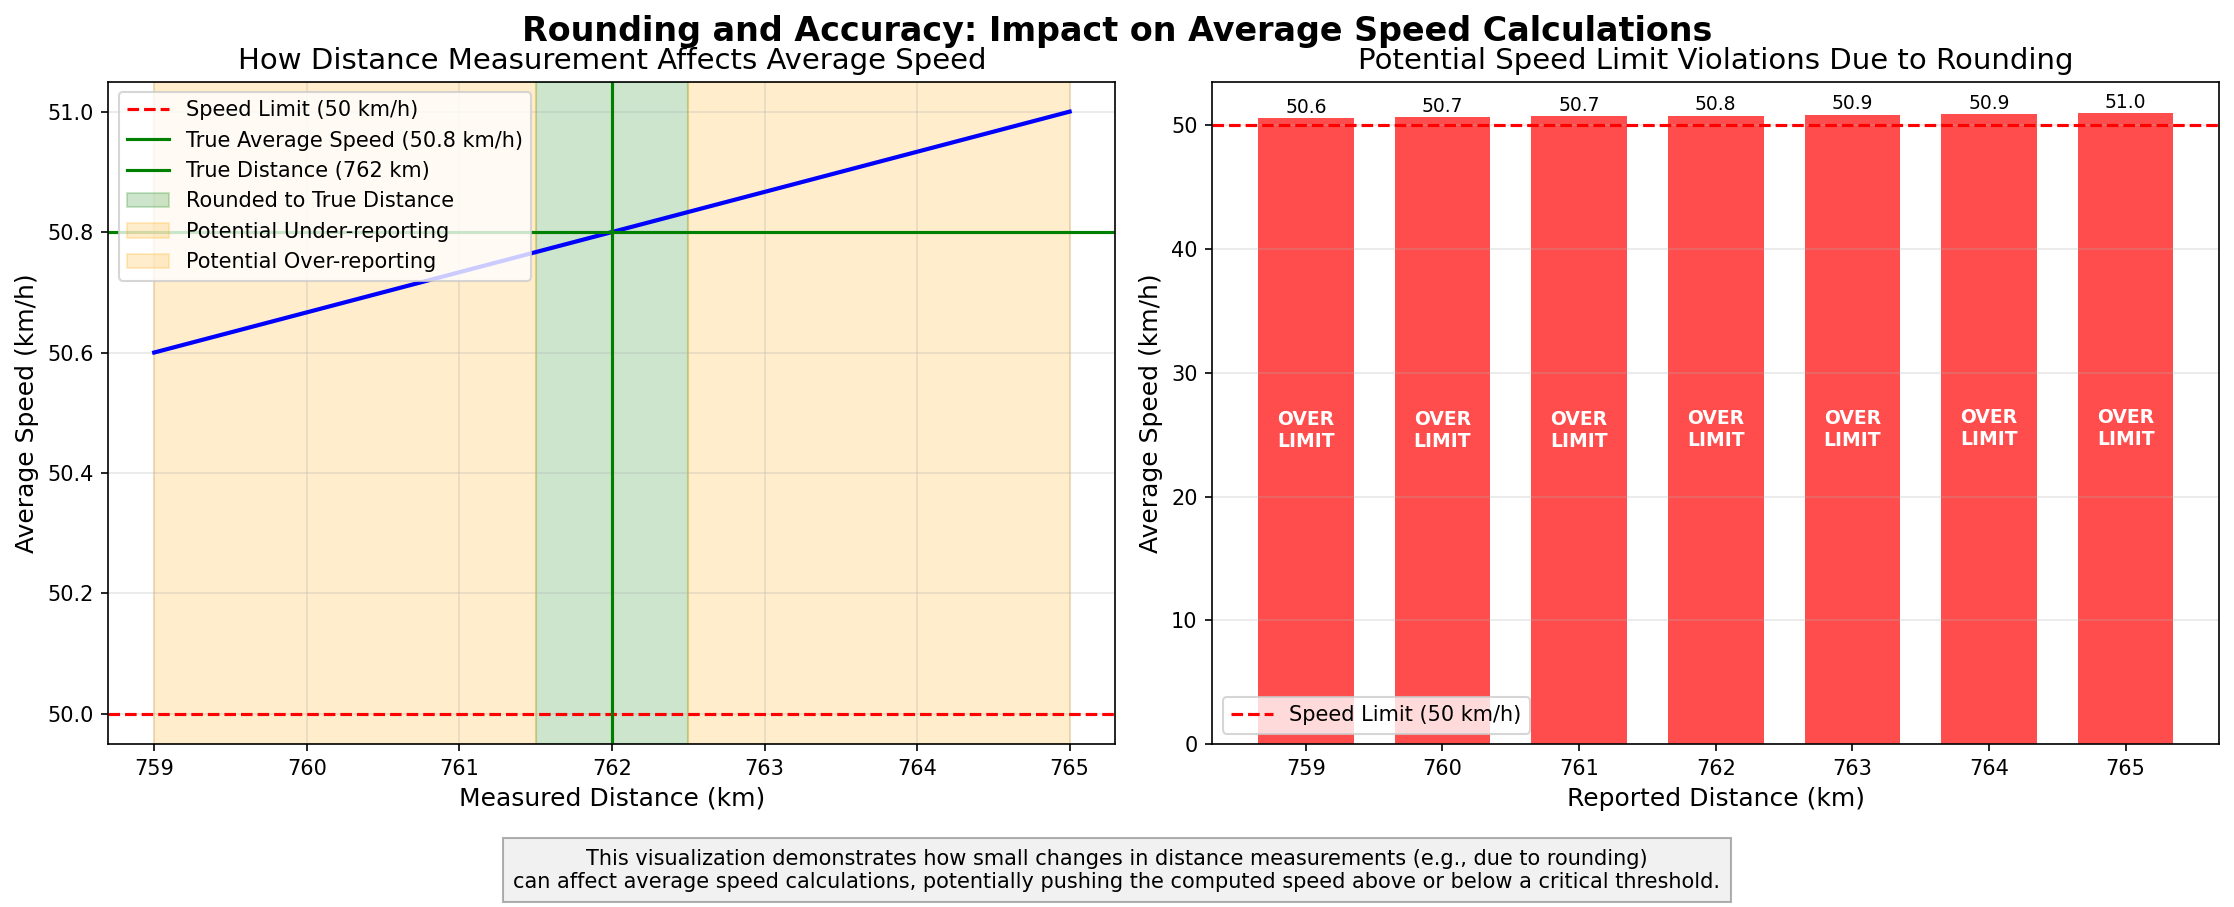
\includegraphics[width=\textwidth]{figures/rounding_accuracy_demo.png}
    \column{0.42\textwidth}
      \begin{itemize}
        \item Distance measurements rounded to nearest kilometer introduce potential error
        \item For our journey: $\dfrac{762\text{ km}}{15\text{ h}} \approx 50.8$ km/h
        \item A mere 3 km error in measurement can push calculated speed above/below the 50 km/h limit
        \item Highlights critical importance of data precision in decision-making applications
      \end{itemize}
  \end{columns}
\end{frame}

% Slide: From Secant to Tangent - The Limit Process
\begin{frame}{From Secant to Tangent: The Limit Process}
  \begin{columns}
    \column{0.5\textwidth}
      \begin{center}
        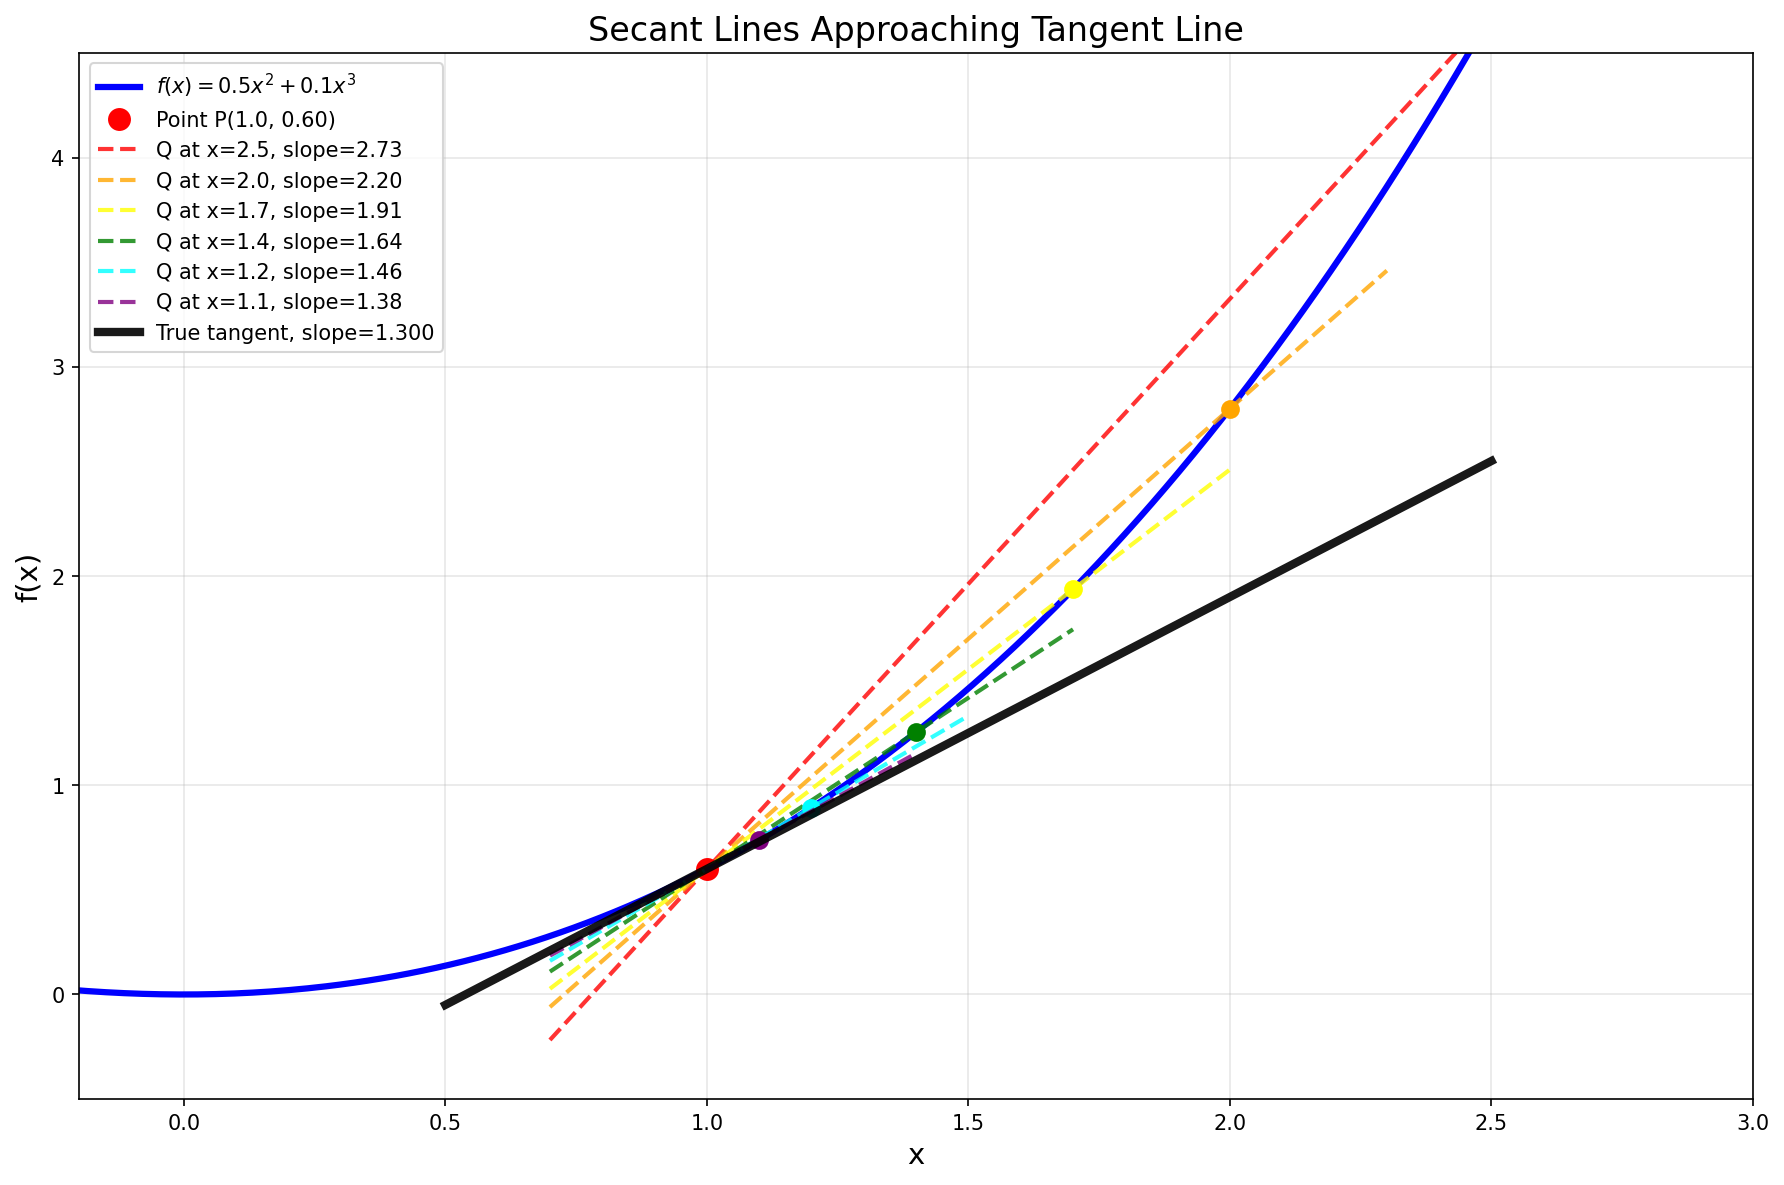
\includegraphics[width=\textwidth]{figures/secant_to_tangent_demo.png}
      \end{center}
    \column{0.5\textwidth}
      \begin{itemize}
        \item As point $Q$ approaches point $P$, secant lines approach the tangent line
        \item Slope of secant: $m_{\text{sec}} = \frac{f(x_1) - f(x_0)}{x_1 - x_0}$
        \item Slope of tangent: $m_{\text{tan}} = \lim_{x_1 \to x_0} \frac{f(x_1) - f(x_0)}{x_1 - x_0}$
        \item This limit gives us the \textbf{derivative} $f'(x_0)$
      \end{itemize}
  \end{columns}
  \vspace{1ex}
  \begin{block}{Key Insights}
    The instantaneous rate of change at a point is the limit of average rates of change as the interval shrinks to zero.
  \end{block}
\end{frame}

% Slide: Average vs Instantaneous Rates
\begin{frame}{Average vs Instantaneous Rates of Change}
  \begin{columns}
    \column{0.5\textwidth}
      \textbf{Average Rate of Change}
      \begin{itemize}
        \item Over an interval $[x_0, x_1]$
        \item Formula: $\frac{f(x_1) - f(x_0)}{x_1 - x_0}$
        \item Geometric: Slope of secant line
        \item Example: Average speed over a trip
      \end{itemize}
    \column{0.5\textwidth}
      \textbf{Instantaneous Rate of Change}
      \begin{itemize}
        \item At a specific point $x_0$
        \item Formula: $f'(x_0) = \lim_{h \to 0} \frac{f(x_0 + h) - f(x_0)}{h}$
        \item Geometric: Slope of tangent line
        \item Example: Speed at exact moment
      \end{itemize}
  \end{columns}
  \vspace{2ex}
  \begin{center}
    \textbf{Connection:} Instantaneous rate = limit of average rates as interval approaches zero
  \end{center}
\end{frame}

% Slide: Toward Instantaneous Rate of Change
\begin{frame}{Instantaneous Rate of Change}
  \begin{itemize}
    \item Instantaneous speed corresponds to slope of tangent line at a point.
    \item As secant interval shrinks ($b\to a$), average rate approaches derivative $f'(x)$.
    \item Next: Formalize tangent lines and derivatives.
  \end{itemize}
\end{frame}
\end{document}